%% ****** Start of file apstemplate.tex ****** %
%%
%%
%%   This file is part of the APS files in the REVTeX 4 distribution.
%%   Version 4.1r of REVTeX, August 2010
%%
%%
%%   Copyright (c) 2001, 2009, 2010 The American Physical Society.
%%
%%   See the REVTeX 4 README file for restrictions and more information.
%%
%
% This is a template for producing manuscripts for use with REVTEX 4.0
% Copy this file to another name and then work on that file.
% That way, you always have this original template file to use.
%
% Group addresses by affiliation; use superscriptaddress for long
% author lists, or if there are many overlapping affiliations.
% For Phys. Rev. appearance, change preprint to twocolumn.
% Choose pra, prb, prc, prd, pre, prl, prstab, prstper, or rmp for journal
%  Add 'draft' option to mark overfull boxes with black boxes
%  Add 'showpacs' option to make PACS codes appear
%  Add 'showkeys' option to make keywords appear
\documentclass[aps,prl,preprint,groupedaddress]{revtex4-1}
%\documentclass[aps,prl,preprint,superscriptaddress]{revtex4-1}
%\documentclass[aps,prl,reprint,groupedaddress]{revtex4-1}

\usepackage{physics}
\usepackage{minted}
\usepackage{graphicx}

% You should use BibTeX and apsrev.bst for references
% Choosing a journal automatically selects the correct APS
% BibTeX style file (bst file), so only uncomment the line
% below if necessary.
%\bibliographystyle{apsrev4-1}

\begin{document}

% Use the \preprint command to place your local institutional report
% number in the upper righthand corner of the title page in preprint mode.
% Multiple \preprint commands are allowed.
% Use the 'preprintnumbers' class option to override journal defaults
% to display numbers if necessary
%\preprint{}

%Title of paper
\title{Variational Monte Carlo methods for nuclear physics}

% repeat the \author .. \affiliation  etc. as needed
% \email, \thanks, \homepage, \altaffiliation all apply to the current
% author. Explanatory text should go in the []'s, actual e-mail
% address or url should go in the {}'s for \email and \homepage.
% Please use the appropriate macro foreach each type of information

% \affiliation command applies to all authors since the last
% \affiliation command. The \affiliation command should follow the
% other information
% \affiliation can be followed by \email, \homepage, \thanks as well.
\author{P. Fasano}
%\email[]{Your e-mail address}
%\homepage[]{Your web page}
%\thanks{}
%\altaffiliation{}
\affiliation{University of Notre Dame}

%Collaboration name if desired (requires use of superscriptaddress
%option in \documentclass). \noaffiliation is required (may also be
%used with the \author command).
%\collaboration can be followed by \email, \homepage, \thanks as well.
%\collaboration{}
%\noaffiliation

\date{\today}

\begin{abstract}
Solving the quantum-mechanical many-body problem is a computationally intensive
task due to the high-dimensionality of the position space, as well as the number
of spin and isospin degrees of freedom. Variational Monte Carlo is a technique
for evaluating the high-dimension integrals required by the variational principle.
A simple example implementation of variational Monte Carlo is presented.
\end{abstract}

% insert suggested PACS numbers in braces on next line
\pacs{}
% insert suggested keywords - APS authors don't need to do this
%\keywords{}

%\maketitle must follow title, authors, abstract, \pacs, and \keywords
\maketitle

% body of paper here - Use proper section commands
% References should be done using the \cite, \ref, and \label commands
\section{Introduction}
% Put \label in argument of \section for cross-referencing
%\section{\label{}}
\subsection{Ab Initio Nuclear Theory}

Atomic nuclei are complex many-body systems showing a wide variety of phenomena
and behaviors. \textit{Ab inito} theory methods attempt to predict these phenomena
from the underlying interactions between nucleons. In principle, one would like
to begin with the fundamental quark degrees of freedom described by quantum
chromodynamics (QCD); however, low energy QCD is extremely non-perturbative and
is computationally infeasible for all but the smallest composite systems. Instead,
one begins with realistic nucleon-nucleon (NN) and three-nucleon (3N) interactions
which capture the essential physics necessary for describing nuclei. These interactions
can be constructed in a variety of ways, often guided by the underlying symmetries
of QCD such as with chiral effective field theory \(\chi\)EFT \cite{RevModPhys.87.1067}.
Usually such potentials are fitted to a combination of nucleon-nucleon scattering
data as well as selected nuclear binding energies. Phenomenological potentials
such as the Argonne \(v18'\) potential are able to describe the structure of light
nuclei with great precision.

\subsection{Variational Principle}
The quantum mechanical variational principle states that for any trial wave function
\(\ket{\Psi_T}\), the expectation value
\[\ev{H} = \frac{\ev{H}{\Psi_T}}{\braket{\Psi_T}} \geq E_0\]
where \(E_0\) is the ground-state energy of the Hamiltonian \(H\). The best approximation
to the lowest energy eigenvalue \(E_0\) and ground state wave function \(\ket{\Psi_0}\)
is determined by taking the variation of \(\ev{H}\) and setting it equal to zero
\[\delta \ev{H} = \delta \qty(\frac{\ev{H}{\Psi_T}}{\braket{\Psi_T}}) = 0\]
Approximating the wave function and its ground state energy then consists of varying
some parameters in \(\ket{\Psi_T}\) and finding the minimum.

For many-body systems, calculating the expectation value \(\ev{H}\) involves integrating
over \(3A\) spatial dimensions (where \(A\) is the number of particles) as well as
summing over all spin and isospin degrees of freedom. For traditional methods such
as Simpson's rule or Gaussian quadrature, the error goes as \(O(N^{-k/(3A)})\)
\cite{hjorth-jensen_2013}. This exponential growth means that numerical integration
with such techniques rapidly becomes computationally infeasible as the number of
particles grows. In order to evaluate these integrals, one usually turns to Monte
Carlo techniques; this class of methods samples an integrand at a large number of
random points in space and relates the average of the integrand to the value of
the integral via the mean value theorem
\begin{equation*}
  \int_a^b f(x) g(x) dx = \expval{f} \int_a^b g(x) dx
\end{equation*}
This can be rewritten in a more useful form for Monte Carlo integration
\begin{equation*}
    \int_a^b f(x) g(x) dx \approx \frac{1}{N} \sum_{i=1}^N f(X_i), \quad X_i \in \{g(x)\}
\end{equation*}
where the function \(f(x)\) is sampled at points \(X_i\) drawn from the probability
distribution \(g(x)\). This converges as \(O^{-1/2}\) regardless of dimensionality
\cite{hjorth-jensen_2013}; thus, Monte Carlo integration is the ideal choice for
integrals over high-dimension spaces.

To evaluate the expectation value \(\ev{H}\), we define the \textit{local energy
operator} \[\vu{E}_L (\vb{r}) = \frac{1}{\Psi_T (\vb{r})} \vu{H} \Psi_T (\vb{r})\]
and probability distribution function
\[P(\vb{r}) = \frac{\qty|\Psi_T(\vb{r})|^2}{\int \qty|\Psi_T(\vb{r})|^2 d \vb{r}}\]
giving us
\[\ev{H} = \int P(\vb{r}) \vu{E}_L (\vb{r}) d \vb{r} \approx
  \frac{1}{N} \sum_{i=1}^N \vu{E}_L (\vb{r}_i), \quad \vb{r}_i \in \{P(\vb{r})\}\]
Thus, to calculate the estimate of the energy for the state \(\ket{\Psi_T}\), we
average the value of the local energy at points selected from a probability distribution
proportional to \(\braket{\Psi_T}\).

\subsection{Metropolis Algorithm}
In general, \(P(\vb{r})\) is not readilty available because the value of the
normalization constant would require doing an integral over the whole space.
The Metropolis algorithm gives a way of sampling random values from an unknown
probability distribution \(P(\vb{r})\) as long as some function \(G(\vb{r}) \sim
P(\vb{r)}\) is known.

To generate the sequence of points at which we sample the local energy, we follow
a random walk through the space:
\subsection{Generating random numbers from a random walk}
\begin{enumerate}
\item Begin with a point \(\vb{r}_i\). Propose \(\vb{r}_{i+1}=\vb{r}_i+\delta \vb{\xi}\)
      where \(\xi_k \in [0,1)\).
\item Calculate \(R = \frac{G(\vb{r}_{i+1})}{G(\vb{r}_i)}\);
\begin{itemize}
    \item if \(R \geq 1\), accept the proposal for \(\vb{r}_{i+1}\),
    \item if \(r < 1\), generate another random number \(\zeta \in [0,1)\) and
          accept proposal if \(\zeta < R\), otherwise set \(\vb{r}_{i+1} = \vb{r}_i\).
\end{itemize}
\item Use \(X_i\) to calculate the value of the integrand \(f(X_i)\).
\end{enumerate}
In effect, the sequence \(\vb{r}_i\) takes a random walk, always accepting moves
to areas with greater probability density, but always having some chance of
moving to areas with lower probability density. It can be shown \cite{kalos_whitlock_2008}
that as \(N \rightarrow \infty\), the sequence \(\{\vb{r}_1,\dots,\vb{r}_N\}\)
will be be randomly sampled from \(P(\vb{r})\).

\section{Nuclear Wave Functions}
The most important task when performing a VMC calculation is selection of an
appropriate trial wave function. For nuclear physics one usually chooses a wave
function factored into a short-range correlation and long-range structure form
\cite{RevModPhys.87.1067,hjorth-jensen_2013}
\[ \ket{\Psi_T} = \qty(\prod_{i<j} f(r_{ij})) \ket{\Phi} \]
where \(r_{ij}\) is the distance between the \(i\)th and \(j\)th particle. Since
the behavior of two nucleons close together is dominated by the NN-interaction
between them, the functions \(f(r_{ij})\) satisfy the one-dimensional
Schr\"{o}dinger equation
\[ \qty(-\frac{\hbar^2}{2\mu} \dv[2]{r_{ij}} + q V(r_{ij})) f(r_{ij}) = \epsilon f(r_{ij}) \]
where \(q\) is a variational parameter adjusting the strength of the short-range
interaction, and a boundary condition is imposed such that \(f(r_{ij})\) is
constant beyond \(r_{ij} > h\) where \(h\) is another variational parameter
controlling the range of the correlation.

The long-range structure \(\ket{\Phi}\) is an antisymmetric function which captures
the behavior of the nucleons when separated at larger distances. Often \(\ket{\Phi}\)
is chosen to be a single Slater determinant or sum of Slater determinants.

An additional simplification can be made for nuclear Hamiltonians which are
spin-independent: we may additionally factor the Slater determinants into
\cite{pederiva_roggero_schmidt_2016}
\[ \Phi = \det[\phi_{p_i \uparrow}] \det[\phi_{p_i \downarrow}]
\det[\phi_{n_i \uparrow}] \det[\phi_{n_i \downarrow}] \]

\section{Computational Implementation and Preliminary Results}
The algorithms above were implemented in C++11. Random numbers are generated the
Intel Math Kernel Library with the Mersenne-Twister pseudorandom number
generator algorithm. The Metropolis algorithm has an adaptive step size, and
attempts to hit a particular acceptance rate target; if the acceptance rate is
too high, it is likely that the step size is too small, leading to correlations
between nearby sample points, while an acceptance rate too low implies that the
step often tries to move to areas of very small probability density. Wave
functions are implemented as subclasses of \mintinline{cpp}{wf::WaveFunction}.
Each wave function class is expected to provide \mintinline{cpp}{value(r)},
\mintinline{cpp}{local_grad(r)}, \mintinline{cpp}{local_laplacian(r)} and can
optionally override \mintinline{cpp}{norm(r)}, \mintinline{cpp}{grad(r)}, and
\mintinline{cpp}{laplacian(r)}.

For the simplest test case, a ground-state harmonic oscillator wave function is
provided by \mintinline{cpp}{wf::SphericalOscillatorWF}, representing
\[ \phi(\vb{r}) = e^{-r^2/2b^2} \]
Potentials are defined by the \mintinline{cpp}{potential::Potential} class and
are expected to override \mintinline{cpp}{operator()} to accept the state and
return a potential energy. \mintinline{cpp}{potential::HarmonicOscillator} represents
\[ V(\vb{r}) = \frac{\hbar^2}{2 m} \frac{r^2}{b^4} \]

This object-oriented structure allows for having a general framework in which
VMC calculations can be done, both for one-body and many-body systems. Shown
in the figures are energies as a function of wave function length parameter for
a harmonic oscillator and an anharmonic oscillator (\(V(r) \sim r^4\)).

\begin{figure}
  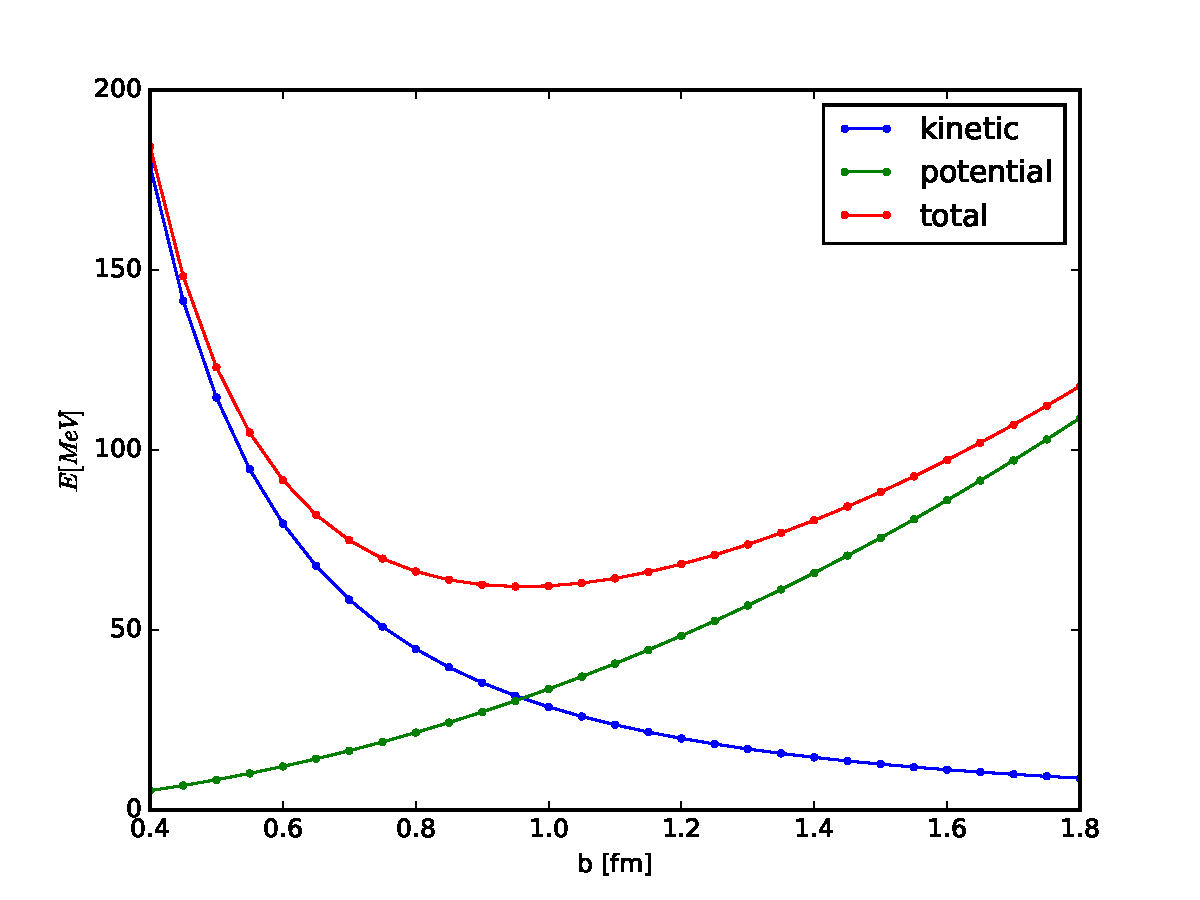
\includegraphics[width=0.8\linewidth]{figure_1.pdf}
  \caption{Variational energy as a function of oscillator length for the
    harmonic oscillator.}
\end{figure}
\begin{figure}
  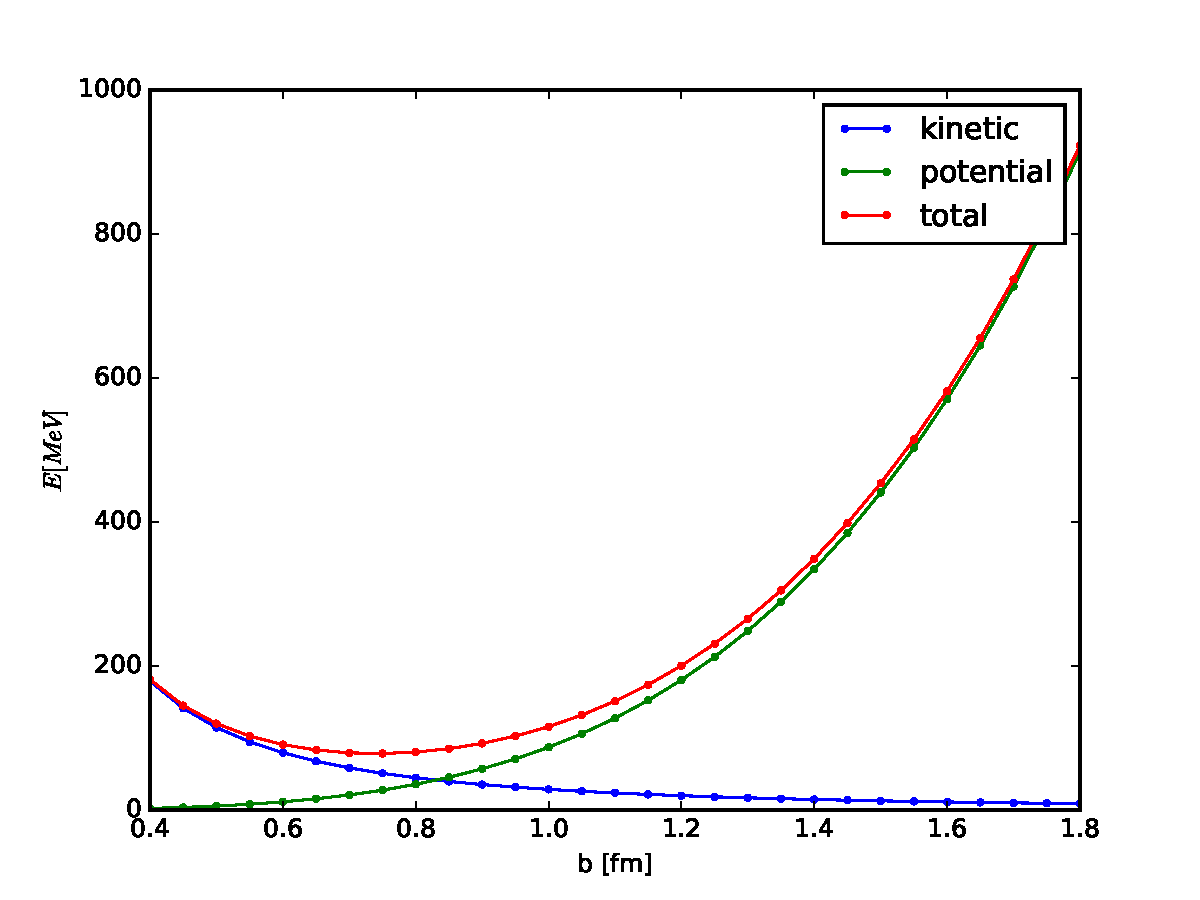
\includegraphics[width=0.8\linewidth]{figure_2.pdf}
  \caption{Variational energy as a function of oscillator length for the
    anharmonic oscillator.}
\end{figure}


%\subsubsection{}

% If in two-column mode, this environment will change to single-column
% format so that long equations can be displayed. Use
% sparingly.
%\begin{widetext}
% put long equation here
%\end{widetext}

% figures should be put into the text as floats.
% Use the graphics or graphicx packages (distributed with LaTeX2e)
% and the \includegraphics macro defined in those packages.
% See the LaTeX Graphics Companion by Michel Goosens, Sebastian Rahtz,
% and Frank Mittelbach for instance.
%
% Here is an example of the general form of a figure:
% Fill in the caption in the braces of the \caption{} command. Put the label
% that you will use with \ref{} command in the braces of the \label{} command.
% Use the figure* environment if the figure should span across the
% entire page. There is no need to do explicit centering.

% \begin{figure}
% \includegraphics{}%
% \caption{\label{}}
% \end{figure}

% Surround figure environment with turnpage environment for landscape
% figure
% \begin{turnpage}
% \begin{figure}
% \includegraphics{}%
% \caption{\label{}}
% \end{figure}
% \end{turnpage}

% tables should appear as floats within the text
%
% Here is an example of the general form of a table:
% Fill in the caption in the braces of the \caption{} command. Put the label
% that you will use with \ref{} command in the braces of the \label{} command.
% Insert the column specifiers (l, r, c, d, etc.) in the empty braces of the
% \begin{tabular}{} command.
% The ruledtabular enviroment adds doubled rules to table and sets a
% reasonable default table settings.
% Use the table* environment to get a full-width table in two-column
% Add \usepackage{longtable} and the longtable (or longtable*}
% environment for nicely formatted long tables. Or use the the [H]
% placement option to break a long table (with less control than
% in longtable).
% \begin{table}%[H] add [H] placement to break table across pages
% \caption{\label{}}
% \begin{ruledtabular}
% \begin{tabular}{}
% Lines of table here ending with \\
% \end{tabular}
% \end{ruledtabular}
% \end{table}

% Surround table environment with turnpage environment for landscape
% table
% \begin{turnpage}
% \begin{table}
% \caption{\label{}}
% \begin{ruledtabular}
% \begin{tabular}{}
% \end{tabular}
% \end{ruledtabular}
% \end{table}
% \end{turnpage}

% Specify following sections are appendices. Use \appendix* if there
% only one appendix.
%\appendix
%\section{}

% If you have acknowledgments, this puts in the proper section head.
%\begin{acknowledgments}
% put your acknowledgments here.
%\end{acknowledgments}

% Create the reference section using BibTeX:
\bibliography{vmc}

\end{document}
%
% ****** End of file apstemplate.tex ******
